\documentclass[11pt, a4paper, oneside]{exam}
\usepackage[margin=3cm]{geometry}
\usepackage{amsmath}
\usepackage{amsthm}
\usepackage{amsfonts}
\usepackage{MnSymbol}
\usepackage{appendix}
\usepackage{graphicx}

\theoremstyle{definition}\newtheorem{define}{Definition}[section]
\theoremstyle{remark}\newtheorem{remark}{Remark}
\theoremstyle{definition}\newtheorem{example}{Example}[subsection]
\theoremstyle{definition}\newtheorem{notation}{Notation}[section]
\theoremstyle{definition}\newtheorem{theorem}{Theorem}[section]
\theoremstyle{definition}\newtheorem{corollary}{Corollary}[section]

\usepackage{tikz, pgf}


\title{asdf}
\author{Name
}
\date{}

\begin{document}
\section{Solutions to Proof Questions}
\begin{enumerate}
\item 

If the floor is wet then it is raining.

\item 

\begin{itemize}
  \item The city of Toronto is in Australia.
  \item The weather is good and I will not be at the beach.
  \item Let $U$ be the set of even numbers. The statement is therefore represented by the following syntax:
    \[ \forall x \in U, \forall k \in \mathbb{Z}, kx \in U \]
    The negation of this, is therefore:
    \[ \exists x \in U, \exists k \in \mathbb{Z}, kx \not \in U \]
    Converting this back to English:

    There exists multiples of even numbers that are not even.
\end{itemize}

\item 

If a polygon does not have an angle sum of $360\circ$ then it is not a square.

\item

\begin{itemize}
\item If a number is odd then it does not have a remainder of 0 when divided by 2.
\item If a number does not have a remainder of 0 when divided by 2 then it is odd.
\end{itemize}

\item Let the three consecutive odd integers be $k-2$, $k$ and $k+2$ where $k$ is an odd integer. Then the sum is equal to $(k-2) + k + (k+2) = 3k$, which is divisible by 3.

\item Prove that a positive integer that ends in 325 cannot be the square of an integer.

In order for the square of an integer to end in 5, the last digit of the integer must be 5. Exhaustively listing all possibilities:
\begin{align*}
(\ldots05)^2 & = \ldots025\\
(\ldots15)^2 & = \ldots225\\
(\ldots25)^2 & = \ldots625\\
(\ldots35)^2 & = \ldots225\\
(\ldots45)^2 & = \ldots025\\
(\ldots55)^2 & = \ldots025\\
(\ldots65)^2 & = \ldots225\\
(\ldots75)^2 & = \ldots625\\
(\ldots85)^2 & = \ldots225\\
(\ldots95)^2 & = \ldots025
\end{align*}
Hence, a square of an integer cannot end in 325.



\item The contrapositive is to prove for an integer $n$, if $n$ is not divisible by 3 then $n^2-1$ is divisible by 3.

There are two cases for $n$ not to be divisible by 3:

\textbf{Case 1: $n = 3k +1$ for some $k \in \mathbb{Z}$}
\begin{align*}
n^2 -1 & = (3k+1)^2 - 1\\
& = 9k^2 + 6k + 1 -1 \\
& = 9k^2 + 6k\\
& = 3(3k^2 + 2k)
\end{align*}
As the integers are closed under the operations of addition and multiplication, then $n^2-1$ is divisible by 3.

\textbf{Case 2: $n = 3k +2$ for some $k \in \mathbb{Z}$}
\begin{align*}
n^2 -1 & = (3k+2)^2 - 1\\
& = 9k^2 + 6k + 4 -1 \\
& = 9k^2 + 6k + 3\\
& = 3(3k^2 + 2k + 1)
\end{align*}
As the integers are closed under the operations of addition and multiplication, then $n^2-1$ is divisible by 3.

Hence, we have proven that if $n$ is not divisible by 3 then $n^2-1$ is divisible by 3.

\item 
\begin{enumerate}
\item Show by expanding that 

\[x^n -1 = (x-1)(x^{n-1} + x^{n-2} + x^{n-3} + \ldots + x^2 + x + 1) \]

\item By proving the contrapositive, prove that if $2^n - 1$ is a prime number, then $n$ is also prime.
\item Give a counter-example of the converse.

\end{enumerate}

\begin{enumerate}
\item 
\begin{align*}
& (x-1)(x^{n-1} + x^{n-2} + x^{n-3} + \ldots + x^2 + x + 1)\\
& = (x^n + x^{n-1} + x^{n-2} + \ldots + x^3 + x^2 + x)\\
& \quad\quad - (x^{n-1} + x^{n-2} + \ldots + x^3+ x^2 + x + 1)\\
& = x^n - 1
\end{align*}
\item We prove the contrapositive statement: If $n$ is not prime then $2^n-1$ is not a prime number.

For $n$ not to be prime, then there exists $p,q \in\mathbb{Z}$ such that $n = pq$.
\begin{align*}
2^n - 1 & = 2^{pq} - 1\\
& = (2^p)^q - 1 \\
& = (2^p - 1)(2^{p(q-1)} + 2^{p(q-2)} + 2^{p(q-3)} + \ldots + 2^{3p} +  2^{2p} + 2^p + 1)
\end{align*}
Due to the closure of the integers under multiplication and addition, then we have proven that $2^n - 1$ can be factorised into the product of two integers. Hence, it is not prime.

\end{enumerate}






\item Prove that for an integer $n$, if $n^2 - 6n + 5$ is even then $n$ is odd.


Suppose by contradiction that for an integer $n$, if $n^2 - 6n +5$ is even then $n$ is even.

\begin{align*}
n^2 - 6n + 5 & = (n-5)(n-1)
\end{align*}
Since $n$ is even, then $n-5$ and $n-1$ are odd. The product of two odd numbers is also odd, which is a contradiction.

\item

Suppose by contradiction that $\cos^2(5^\circ)$ is rational.

\begin{align*}
\Rightarrow & \cos^2(5^\circ) = \frac{\cos (10^\circ) + 1}{2} \mbox{ is rational }\\
\Rightarrow & \cos (10^\circ) \mbox{ is rational }\\
\Rightarrow & \cos (10^\circ) = \frac{4\cos^3 (10^\circ) - \cos (30^\circ)}{3}\mbox{ is rational}\\
\Rightarrow & \cos(30^\circ) \mbox{ is rational}
\end{align*}
However, $\cos(30^\circ) =\frac{\sqrt{3}}{2}$ which is irrational. This is a contradiction, hence $\cos^2(5^\circ)$ is irrational.

\item

Since $n$ is a composite integer, it has a factor $a,b$ with $1<a<n$ and $1<b<n$ such that $|n| = ab$.

If $a > \sqrt{n}$ and $b > \sqrt{n}$ then $ab > \sqrt{n} \times \sqrt{n} = n$ which is a contradiction.

Hence, $a \leq \sqrt{n}$ or $b \leq \sqrt{n}$.

Since $a$ and $b$ are factors of $n$ then we can see that $n$ has a positive factor not greater than $\sqrt{n}$. This factor is either a prime number or, it has a prime factor less than itself. In both cases, $n$ therefore has a prime divisor $\leq \sqrt{n}$.







%%%%%%%%

\item %Prove by induction \[ \sum_{r=1}^n r(3r-1) = n^2(n+1) \]


Let $S(n)$ be $ \sum_{r=1}^n r(3r-1) = n^2(n+1)$.

For $n=1$:
\begin{align*}
LHS & =  \sum_{r=1}^1 r(3r-1)\\
& = 1(3-1)\\
& = 2\\
\\
RHS & = (1)^2(1+1)\\
& = 2\\
\\
LHS & = RHS
\end{align*}
Therefore $S(1)$ is true.

Assume $S(k)$ to be true for some $k \in \mathbb{Z}$. i.e. $ \sum_{r=1}^k r(3r-1) = k^2(k+1)$

We are required to prove $S(k+1)$ to be true.
\begin{align*}
LHS & =  \sum_{r=1}^{k+1} r(3r-1)\\
& =  \sum_{r=1}^k r(3r-1) + (k+1)(3(k+1)-1)\\
& = k^2(k+1) + (k+1)(3k+2) \mbox{ (by the assumption)}\\
& = (k+1)(k^2 + 3k + 2)\\
& = (k+1)(k+1)(k+2)\\
& = (k+1)^2(k+2)\\
& = RHS
\end{align*}

By the principle of Mathematical induction, $S(n)$ is true for $n \in \mathbb{Z}^+$.

\item %A sequence is recursively defined by $a_1 = 3$ and $a_n = 2a_{n-1} - 1$ for $n >1$. Prove by induction that $a_n = 2^n + 1$.\\

  Let $S(n)$ be: if a recursive sequence is defined by $a_1 = 3$ and $a_n = 2a_{n-1} - 1$ for $n >1$, then $a_n = 2^n + 1$.

\begin{align*}
  a_1 = 2^1 + 1 = 3
\end{align*}
Therefore $S(1)$ is true.

Assume $S(k)$ is true for some $k \in \mathbb{Z}$. i.e. $a_k = 2^k + 1$.

We are required to prove $S(k+1)$ is true.
\begin{align*}
  a_{k+1} & = 2a_{k} - 1\\
          & = 2(2^k + 1) -1\\
          & = 2^{k+1} + 2 - 1\\
          & = 2^{k+1} + 1
\end{align*}
Hence, true for $S(k+1)$.

By the principle of Mathematical Induction, $S(n)$ is true for $n \in \mathbb{Z}^+$.



\item %Prove by induction for all positive integers $n$ that $5^n + 2\times11^n$ is divisible by 3.

Let $S(n)$ be ``$5^n + 2\times 11^n$ is divisible by $3$ for all $n\in\mathbb{Z}^+$.

Test $n = 1$:
\begin{align*}
LHS & = 5^1 + 2\times 11^1 \\
& = 5 + 22\\
& = 27\mbox{ which is divisible by 3}
\end{align*}
Therefore $S(1)$ is true.

Assume $S(k)$ is true for some $k \in\mathbb{Z}$. i.e. Let $5^k + 2\times 11^k = 3M$ for some $M \in \mathbb{Z}$.

We are required to prove $S(k+1)$ is true.

\begin{align*}
LHS & = 5^{k+1} + 2\times 11^{k+1}\\
& = 5\times5^k + 2\times11\times11^k\\
& = 5\times 5^k + 5 \times 2\times 11^k - 5 \times 2\times 11^k + 2\times 11 \times 11^k\\
& = 5(5^k + 2\times 11^k) + (-10 + 22)\times 11^k\\
& = 5(3M) + 12\times 11^k \mbox{ (By the assumption)}\\
& = 3(5M + 4\times 11^k) \mbox{ which is divisible by 3}
\end{align*}
Therefore, $S(k+1)$ is true.

By the principle of Mathematical induction, $S(n)$ is true for $n \in \mathbb{Z}^+$.

\item %Prove by induction $n! > 2^n$ for integers $n\geq 4$.

Let $S(n)$ be ``$n! > 2^n$ for integers $n \geq 4$.''

Test $n = 4$:
\begin{align*}
LHS & = 4!\\
 = 24\\
 \\
 RHS & = 2^4 \\
 & = 16\\
 \\
 LHS & > RHS 
\end{align*}
Therefore $S(4)$ is true.

Assume $S(k)$ true, i.e. $k! > 2^k$ for some integer $k \geq 4$.

Required to prove $S(k+1)$ is true.

\begin{align*}
LHS & = (k+1)!\\
& = (k+1)k!\\
& > (k+1) 2^k \mbox{ (by the assumption)}\\
& > 2\times 2^k \mbox{ as $k+1 > 2$ for $k \geq 4$}\\
& = 2^{k+1}\\
& = RHS
\end{align*}
Hence, true for $S(k+1)$.

By the principle of Mathematical induction, $S(n)$ is true for $n \in \mathbb{Z}, n \geq 4$.




\item
\begin{enumerate}
\item 
\begin{align*}
(x-y)^2 & \geq 0\\
x^2 - 2xy + y^2 & \geq 0\\
x^2 + y^2 & \geq 2xy
\end{align*}
\item
From part a), $a^2 + b^2 = 1 \geq 2ab$ and $c^2 + d^2 = 1 \geq 2cd$.

Hence, $\frac{1}{2} \geq ab$ and $\frac{1}{2} \geq cd$. Adding these together, we obtain the necessary result.
\end{enumerate}




\item By using the AM-GM inequality, show that for all positive integers $n$, 
\[ n! \leq \left(\frac{n+1}{2}\right)^n \]

Apply the AM-GM inequality to the numbers $1,2,3,\ldots,n-1,n$.

\begin{align*}
\sqrt[n]{n!} & \leq \frac{1+2+3+\ldots+n}{n}\\
& \leq \frac{\frac{n(n+1)}{2}}{n} \mbox{ (Using summation of Arithmetic Series formula)}\\
& \leq \frac{n+1}{2}\\
n! &\leq \left(\frac{n+1}{2}\right)^n
\end{align*}

\item 
\begin{enumerate}
\item


Draw an arbitrary triangle, without loss of generality, in the first quadrant of the number plane with integer coordinates for the vertices. Then project the vertices to the horizontal axis.

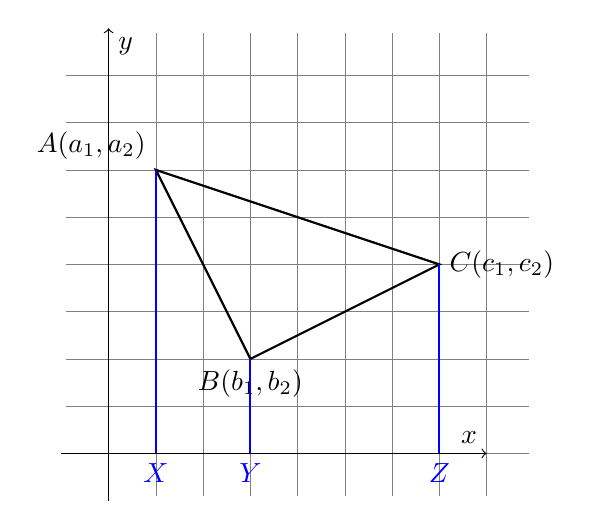
\begin{tikzpicture}[scale=0.6]
\draw[step=1cm,gray,very thin] (-4.9,-4.9) grid (4.9,4.9);
\draw[->] (-4,-5) -- (-4,5) node[anchor=north west] {$y$};
\draw[->] (-5,-4) -- (4,-4) node[anchor=south east] {$x$};

\draw[thick] (-3,2) node[anchor = south east] {$A(a_1, a_2)$} -- (3,0) node[anchor = west] {$C(c_1,c_2)$} -- (-1,-2) node[anchor = north] {$B(b_1,b_2)$} -- cycle;
\draw[blue,thick] (-3,-4) node[anchor = north] {$X$} -- (-3,2);
\draw[blue,thick] (-1,-4) node[anchor = north] {$Y$} -- (-1,-2);
\draw[blue,thick] (3,0) -- (3,-4) node [anchor = north] {$Z$};

\end{tikzpicture}

The area of the triangle is found by subtracting the areas of trapeziums $AXYB$ and $CBYZ$ from $AXZC$.

Hence, 
\begin{align*}
\mbox{Area Triangle} & = \frac{\left|c_1 - a_1\right|}{2}(a_2 + c_2) - \frac{|b_1 - a_1|}{2}(a_2 + b_2) - \frac{|b_1 - c_1|}{2}(b_2 + c_2)
\end{align*}
Since all $a_i,b_i,c_i \in \mathbb{Z}$, it follows that the area of the triangle is rational.


\item

The area of an equilateral triangle with side $x$ is equal to $\frac{1}{2}x^2\sin60^\circ = \frac{\sqrt{3}}{4}x^2$.

Since $\sqrt{3}$ is irrational, then the product of $\sqrt{3}$ with the side lengths $x$ squared, which are rational, will be irrational. Hence, the area will be irrational if the triangle is equilateral.

Therefore, the triangle $ABC$ cannot be an equilateral triangle.




\end{enumerate}



\item
If $R \in R$, then $R$ is a set that is not a member of itself by definition. Hence $R \notin R$.

If $R \notin R$, then the set $R$ must contain this set too as it doesn't contain itself. Hence $R \in R$.




\end{enumerate}


\end{document}















